\documentclass{article}

\usepackage{graphicx}
\usepackage{wrapfig}
\usepackage[margin=2cm,twocolumn]{geometry}

\usepackage{hyperref}
\usepackage[dvipsnames]{xcolor}
\hypersetup{colorlinks=true,urlcolor=MidnightBlue,citecolor=Blue,linkcolor=Blue}

\usepackage[backend=biber,citestyle=numeric]{biblatex}
\addbibresource{/home/nate/Dropbox/nates-biblio-DB.bib}

\linespread{1.2}

\title{Toronto Bike Map \\ Project Prospectus}
\author{Nate Wessel, PhD \\ \href{mailto:bike756@gmail.com}{bike756@gmail.com}}

\begin{document}
	\maketitle
	%Our streets and roads, as they now exist, were built for cars. Cyclists in North America, though growing in numbers, have had almost none of the slow, fluvial influence of a full century of widespread automotivity. Yet in the eddies and on the margins thin tendrils of cycling infrastructure have crept their way into an increasingly fractured rock. The scene is still chaotic, the way forward unclear. 
	
	\section*{Background}
		In the winter of 2014 I began a project to ``rethink the urban bike map.''\cite{Wessel2015} 
		I was living in Cincinnati, Ohio and I had grown frustrated with the maps I could find to help me navigate by bike. One genre of maps, produced locally by our MPO, listed streets which were {\color{ForestGreen}good} or {\color{red}bad} for cycling. As an independent-minded person, this struck me as more than a little condescending, especially as I knew the human source of the these judgments was a single and not singularly representative cyclist.
		Another genre, generally available online, overlaid bike-specific infrastructure on a standard street map. This being not the Netherlands however, that infrastructure was hopelessly fragmented, while the map that remained uncovered was essentially a map for cars\footnote{This seems to be the dominant paradigm in Toronto. E.g. \href{https://www.toronto.ca/services-payments/streets-parking-transportation/cycling-in-toronto/cycling-google-map/}{https://www.toronto.ca/services-payments/streets-parking-transportation/cycling-in-toronto/cycling-google-map/}}.
	
		I decided I would publish my own map, something I had done once a few years before when our local transit agency had failed for several years to create a decent system map on their own.
		My idea was that the new bike map should be thoroughly \textit{objective} and that it also needed to show much more than just the disjunct and miscellaneous bike lanes and cycletracks of other maps. I classified every single street according to its width and speed limit, highlighting those with restricted auto access and lightly emphasizing bike lanes where they existed. Cincinnati has quite a few cul-de-sacs and one of the more innovative ideas I had was to detect these using an algorithm borrowed from graph theory so that these could be de-emphasized relative to other streets.\footnote{
			Tarjan's algorithm for the detection of strongly connected subcomponents. Any edge not belonging to the main strongly connected component was rendered partly transparent.
		} Dead-end signs have always bothered me - a dead end for a car may not be a dead-end for a bike or a pedestrian as indeed it often isn't. Access restrictions on each way were used to define dead-ends \textit{for cyclists}. 
		This cycling-specific measure of network connectivity ended up rather dramatically improving the readability of the map. 
		By spring of 2015, I had printed and distributed the map (9,000 paper copies and online) with the help of a local foundation and several generous sponsors. The project as well as the history and thought behind it have been thoroughly documented in an article in Cartographic Perspectives.\cite{Wessel2015}
		\begin{figure}[h!]
			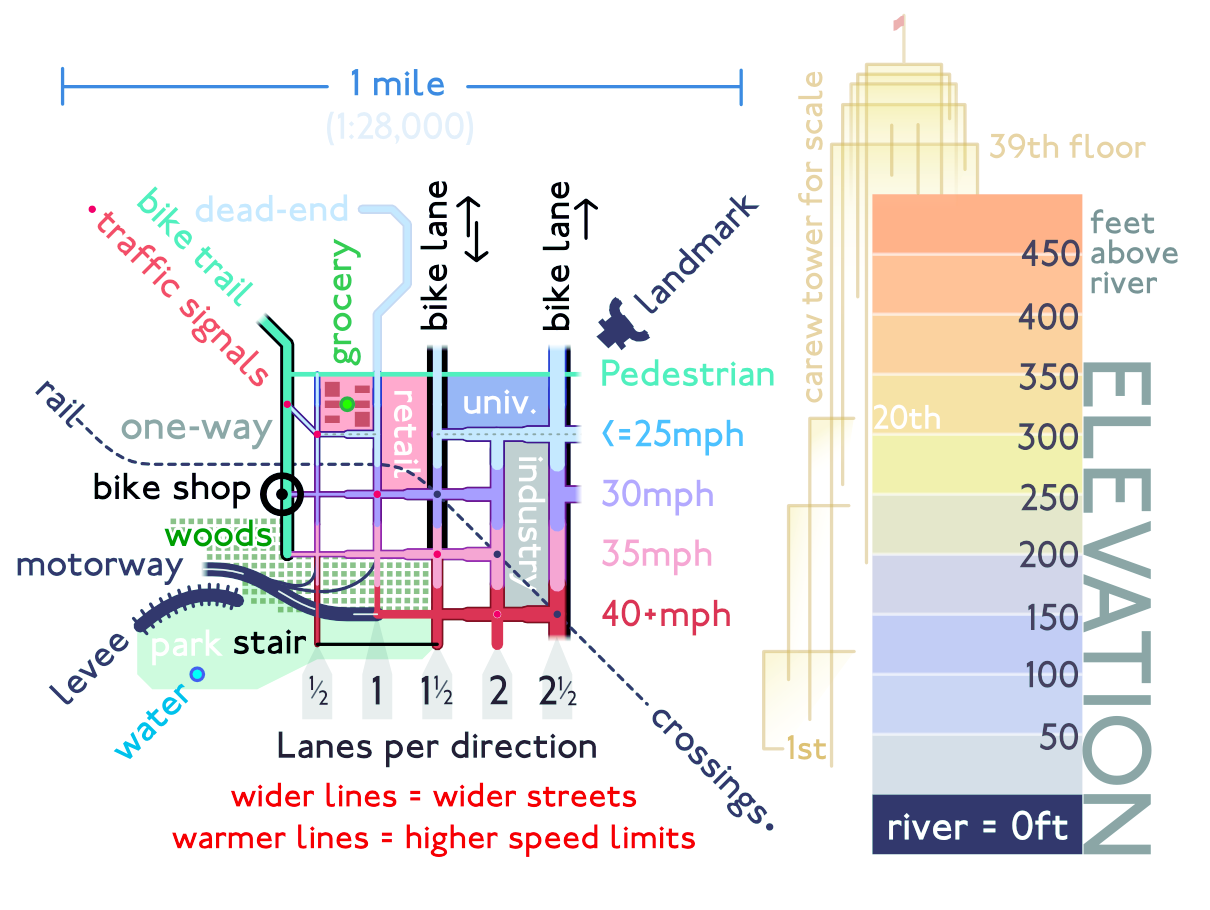
\includegraphics[width=0.48\textwidth]{legend}
			\caption{Legend of the Cincinnati Bike Map}
		\end{figure}
		As I used the new map for actual navigation I began to wonder if there weren't better, more elegant ways of defining connectivity from a cyclist's unique perspective. By mapping road width onto the width of lines on the map, I had introduced a somewhat car-oriented perspective; bigger, busier streets for cars were generally bigger and bolder on my map, regardless of their utility for cyclists. 
		
	\section*{A Second Attempt}
		I had made the first map with data from OpenStreetMap which allows every edge and node to have mode-specific access restrictions. Several advanced route-planning applications exist specifically to use this data to help cyclists plan trips according to their preferences and limitations. I eventually realized that I could use one of these\footnote{
			OSRM, the Open Source Routing Machine: http://map.project-osrm.org/
		} to approximate a measure of \textit{betweenness centrality}\footnote{
			\href{https://en.wikipedia.org/wiki/Betweenness_centrality}{https://en.wikipedia.org/wiki/Betweenness\_centrality}
		}. This concept, borrowed again from graph theory, essentially measures the importance of links in a network by counting the number of least-cost paths across that network to which they belong. By simulating a large and vaguely realistic set of bicycle trips to and from points around the city, I could thus approximate an uncongested flow of cyclists across the city. 
	
\printbibliography
	
\end{document}